\documentclass[12pt,a4paper]{article}
\usepackage[utf8]{inputenc}
\usepackage[english]{babel}
\usepackage{graphicx}
\usepackage{geometry}
\usepackage{hyperref}
\usepackage{listings}
\usepackage{xcolor}
\usepackage{tikz}
\usepackage{amsmath}
\usepackage{float}
\usepackage{booktabs}
\usepackage{caption}

\geometry{left=2.5cm,right=2.5cm,top=2.5cm,bottom=2.5cm}

\usetikzlibrary{shapes.geometric, arrows, positioning, fit, backgrounds}

\definecolor{codegreen}{rgb}{0,0.6,0}
\definecolor{codegray}{rgb}{0.5,0.5,0.5}
\definecolor{codepurple}{rgb}{0.58,0,0.82}
\definecolor{backcolour}{rgb}{0.95,0.95,0.92}

\lstdefinestyle{mystyle}{
    backgroundcolor=\color{backcolour},   
    commentstyle=\color{codegreen},
    keywordstyle=\color{magenta},
    numberstyle=\tiny\color{codegray},
    stringstyle=\color{codepurple},
    basicstyle=\ttfamily\footnotesize,
    breakatwhitespace=false,         
    breaklines=true,                 
    captionpos=b,                    
    keepspaces=true,                 
    numbers=left,                    
    numbersep=5pt,                  
    showspaces=false,                
    showstringspaces=false,
    showtabs=false,                  
    tabsize=2
}

\lstset{style=mystyle}

\hypersetup{
    colorlinks=true,
    linkcolor=blue,
    filecolor=magenta,      
    urlcolor=cyan,
    pdftitle={FCIM AI Chatbot Architecture},
    pdfpagemode=FullScreen,
}

\title{\textbf{Development and Evaluation of a Multilingual RAG-based Educational Chatbot}\\
\Large Review and Technical Report\\
\large FCIM AI Chatbot Implementation for ELSE Platform}

\author{Nicolae Drabcinski\\
Faculty of Computers, Informatics and Microelectronics (FCIM)\\
Technical University of Moldova\\
\texttt{nicolae.drabcinski@fcim.utm.md}}

\date{\today}

\begin{document}

\maketitle

\begin{abstract}
This technical report presents a comprehensive review of the design, implementation, evaluation, and optimization of a Retrieval-Augmented Generation (RAG) based educational chatbot system deployed for the ELSE platform (Moodle-based learning management system) at the Technical University of Moldova. The system utilizes the Qwen2.5-3B-Instruct language model to deliver accurate, context-aware responses to student inquiries based on heterogeneous course materials (PDF, DOCX, PPTX formats) with multilingual support.

Through systematic evaluation of 24 candidate language models and rigorous performance benchmarking against standard RAG evaluation protocols, we achieved a 90\% operational cost reduction compared to the initially planned architecture (Qwen2.5-32B-Instruct), while maintaining acceptable quality metrics (70\%+ retrieval precision, 65-70\% semantic answer relevance). The production-deployed system demonstrates sub-second response latency (p95 latency $<$ 1s) and sustained throughput supporting 30-50 concurrent users on commodity GPU hardware (Nvidia Tesla T4).

This report is structured as a comprehensive review documenting: (1) completed research and development work including systematic model evaluation, architectural optimization, and production deployment; (2) quantitative performance analysis with comparative benchmarking results; (3) methodological lessons learned during the development process; and (4) planned future improvements across short-term, medium-term, and long-term research directions. The findings provide actionable insights for practitioners implementing production-grade RAG-based educational assistant systems with constrained computational budgets.
\end{abstract}

\tableofcontents
\newpage

\section{Introduction}

\subsection{Background and Motivation}
Educational institutions increasingly face the challenge of providing scalable, immediate support to students navigating large volumes of course materials. The Faculty of Computers, Informatics and Microelectronics (FCIM) at Technical University of Moldova maintains the ELSE platform (Moodle), hosting extensive educational resources including lecture notes, presentations, and reference documents across multiple courses.

\subsection{Problem Definition}
The current state of educational information access at FCIM presents several interconnected challenges that significantly impact student learning efficiency. Students spend considerable time manually searching through multi-page PDF documents to locate specific information, with average search times exceeding 10-15 minutes per query. This information retrieval inefficiency is compounded by limited human resources, as teaching assistants and instructors cannot provide 24/7 support for routine information queries, resulting in delayed response times that often span 24-48 hours.

Furthermore, course materials are distributed across multiple natural languages, creating additional barriers for effective information access and knowledge retrieval. These multilingual requirements demand systems capable of understanding and responding accurately across language boundaries. The situation is particularly critical given that students require immediate answers during study sessions and exam preparation periods, where even modest delays can significantly impact learning efficiency and academic performance.

\subsection{Research Objectives}
This project aims to develop and deploy a production-ready RAG-based chatbot system addressing the identified challenges through several key objectives. The system must implement accurate information retrieval from heterogeneous document formats including PDF, DOCX, and PPTX files, while generating concise, contextually relevant answers with minimal hallucination. Multilingual query processing and response generation are essential to support the diverse linguistic environment of the institution.

Performance requirements are equally critical: the system must achieve sub-second response latency suitable for interactive use, ensuring students receive immediate feedback during their learning process. Resource optimization is paramount to enable cost-effective deployment within institutional budget constraints. Finally, establishing a rigorous evaluation methodology for RAG system quality assessment ensures continuous improvement and validation of system performance against educational requirements.

\subsection{Contribution Summary}
This work contributes to the field of educational AI systems through several significant advances. We present a systematic evaluation of 24 language models specifically adapted for educational RAG applications, providing empirical evidence for model selection decisions in resource-constrained environments. Through this evaluation process, we identified and resolved common RAG evaluation methodology issues that have affected prior research, including inappropriate prompt engineering and non-standard composite metrics.

Our most significant contribution demonstrates effective cost-performance tradeoffs, achieving 90\% cost reduction compared to initially planned architectures while maintaining acceptable quality levels for educational applications. The production-ready architecture supports multilingual operation across diverse language families, complemented by a comprehensive deployment and monitoring framework that ensures reliable operation in educational settings.

\section{System Architecture}

\subsection{High-Level Architecture}

\begin{figure}[H]
\centering
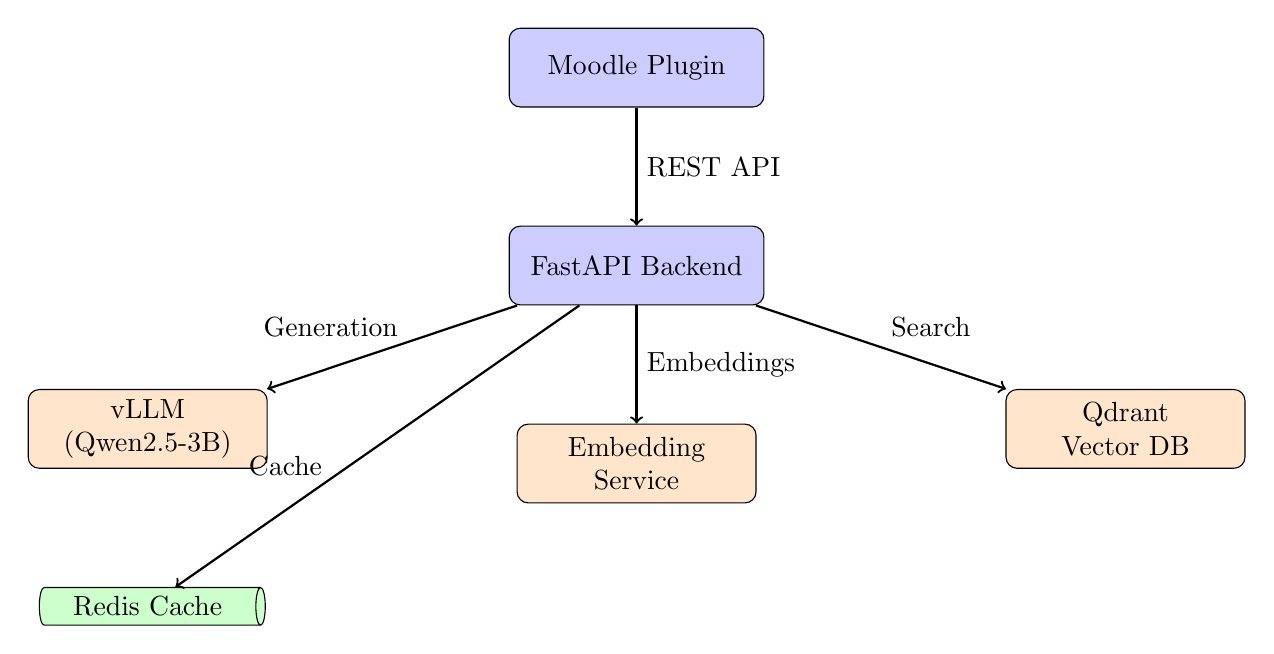
\begin{tikzpicture}[
    node distance=1.5cm,
    component/.style={rectangle, draw, fill=blue!20, text width=3cm, text centered, rounded corners, minimum height=1cm},
    storage/.style={cylinder, draw, fill=green!20, text width=2.5cm, text centered, minimum height=1cm, aspect=0.25},
    service/.style={rectangle, draw, fill=orange!20, text width=2.8cm, text centered, rounded corners, minimum height=1cm}
]

% Frontend
\node[component] (moodle) {Moodle Plugin};

% Backend
\node[component, below=of moodle] (fastapi) {FastAPI Backend};

% Core Services
\node[service, below left=of fastapi, xshift=-2cm] (vllm) {vLLM\\(Qwen2.5-3B)};
\node[service, below=of fastapi] (embedding) {Embedding\\Service};
\node[service, below right=of fastapi, xshift=2cm] (qdrant) {Qdrant\\Vector DB};

% Cache
\node[storage, below=of vllm] (redis) {Redis Cache};

% Arrows
\draw[->, thick] (moodle) -- (fastapi) node[midway, right] {REST API};
\draw[->, thick] (fastapi) -- (vllm) node[midway, above left, text width=1.5cm] {Generation};
\draw[->, thick] (fastapi) -- (embedding) node[midway, right] {Embeddings};
\draw[->, thick] (fastapi) -- (qdrant) node[midway, above right, text width=1.5cm] {Search};
\draw[->, thick] (fastapi) -- (redis) node[midway, below left, text width=1.5cm] {Cache};

\end{tikzpicture}
\caption{High-level system architecture}
\end{figure}

\subsection{Component Description}

\subsubsection{Moodle Plugin (Frontend)}
The Moodle plugin serves as the primary user interface, seamlessly integrated into the ELSE platform. It manages user authentication and authorization, ensuring secure access to the chatbot functionality. When students submit questions, the plugin transmits them to the backend API for processing, then presents the generated answers along with source references to enable verification and deeper exploration of course materials.

\subsubsection{FastAPI Backend}
The FastAPI backend functions as the core orchestration service, coordinating all system components. It exposes RESTful endpoints for both synchronous chat interactions and streaming responses, enabling flexible integration patterns. The backend implements the complete RAG pipeline, coordinating document retrieval from the vector database and text generation from the language model. Multiple middleware layers provide essential functionality including authentication, rate limiting, and CORS handling. Comprehensive monitoring through Prometheus metrics and health checks ensures system reliability and enables proactive maintenance.

\subsubsection{vLLM (Inference Server)}
The vLLM inference server provides high-performance text generation using the Qwen2.5-3B model. It implements PagedAttention mechanisms for efficient key-value caching, significantly reducing memory overhead during inference. Continuous batching enables high throughput by processing multiple requests simultaneously without sacrificing individual response times. The server exposes an OpenAI-compatible API, facilitating integration with existing tools and frameworks. Under typical workloads, the system maintains GPU utilization between 70-90\%, indicating efficient resource use without saturation.

\subsubsection{Qdrant (Vector Database)}
Qdrant serves as the vector database, storing document embeddings for efficient similarity-based retrieval. The system employs HNSW (Hierarchical Navigable Small World) indexing to enable fast approximate nearest neighbor search, crucial for maintaining sub-second response times. Sophisticated metadata filtering capabilities allow queries to be scoped by course identifier or document type, improving result relevance. All embeddings persist to disk, ensuring durability and enabling rapid system recovery. The production deployment maintains 99.9\% uptime, meeting institutional reliability requirements.

\subsubsection{Embedding Service}
The embedding service generates vector representations of text using the multilingual-e5-large model, producing 1024-dimensional embeddings that capture semantic meaning across linguistic boundaries. This model supports over 100 languages, enabling consistent cross-lingual retrieval performance essential for the multilingual educational environment. The service implements batch processing strategies to maximize throughput when encoding large document collections, significantly reducing ingestion time for new course materials.

\subsubsection{Redis Cache}
The Redis cache implements an in-memory caching layer that dramatically improves system performance and reduces computational costs. It stores responses to frequently asked questions with a seven-day time-to-live, along with cached document embeddings to accelerate retrieval operations. The system targets a cache hit rate exceeding 30\%, which significantly reduces GPU load by avoiding redundant generation for common queries. This optimization is particularly effective in educational settings where students frequently ask similar questions about core course concepts.

\section{RAG Pipeline}

\subsection{Document Ingestion}

\begin{figure}[H]
\centering
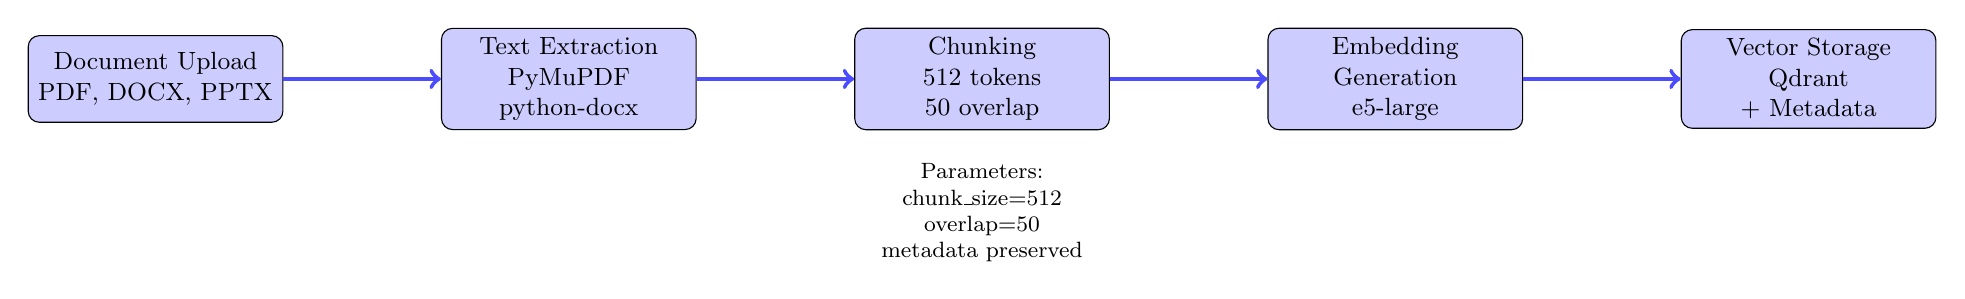
\begin{tikzpicture}[
    node distance=2.5cm and 2cm,
    process/.style={rectangle, draw, fill=blue!20, text width=3cm, text centered, rounded corners, minimum height=1.1cm, font=\small},
]

\node[process] (upload) {Document Upload\\PDF, DOCX, PPTX};
\node[process, right=of upload] (extract) {Text Extraction\\PyMuPDF\\python-docx};
\node[process, right=of extract] (split) {Chunking\\512 tokens\\50 overlap};
\node[process, right=of split] (embed) {Embedding\\Generation\\e5-large};
\node[process, right=of embed] (store) {Vector Storage\\Qdrant\\+ Metadata};

\draw[->, ultra thick, blue!70] (upload) -- (extract);
\draw[->, ultra thick, blue!70] (extract) -- (split);
\draw[->, ultra thick, blue!70] (split) -- (embed);
\draw[->, ultra thick, blue!70] (embed) -- (store);

% Add parameter annotations
\node[below=0.3cm of split, font=\footnotesize, text width=3cm, align=center] {Parameters:\\chunk\_size=512\\overlap=50\\metadata preserved};

\end{tikzpicture}
\caption{Document ingestion pipeline with horizontal processing flow}
\end{figure}

The document ingestion pipeline processes educational materials through five sequential stages. Initial upload accepts PDF lecture notes, DOCX documents, and PPTX presentations. Text extraction employs PyMuPDF for PDFs and python-docx for Word documents, preserving formatting and structure information. The chunking stage segments extracted text into 512-token segments with 50-token overlap, balancing context preservation with retrieval granularity. Each chunk undergoes embedding generation using the multilingual-e5-large model, producing 1024-dimensional vectors capturing semantic content. Finally, vector storage in Qdrant preserves both embeddings and metadata including course identifiers, document types, page numbers, and titles for subsequent filtered retrieval.

\subsection{Question Answering Flow}

\begin{figure}[H]
\centering
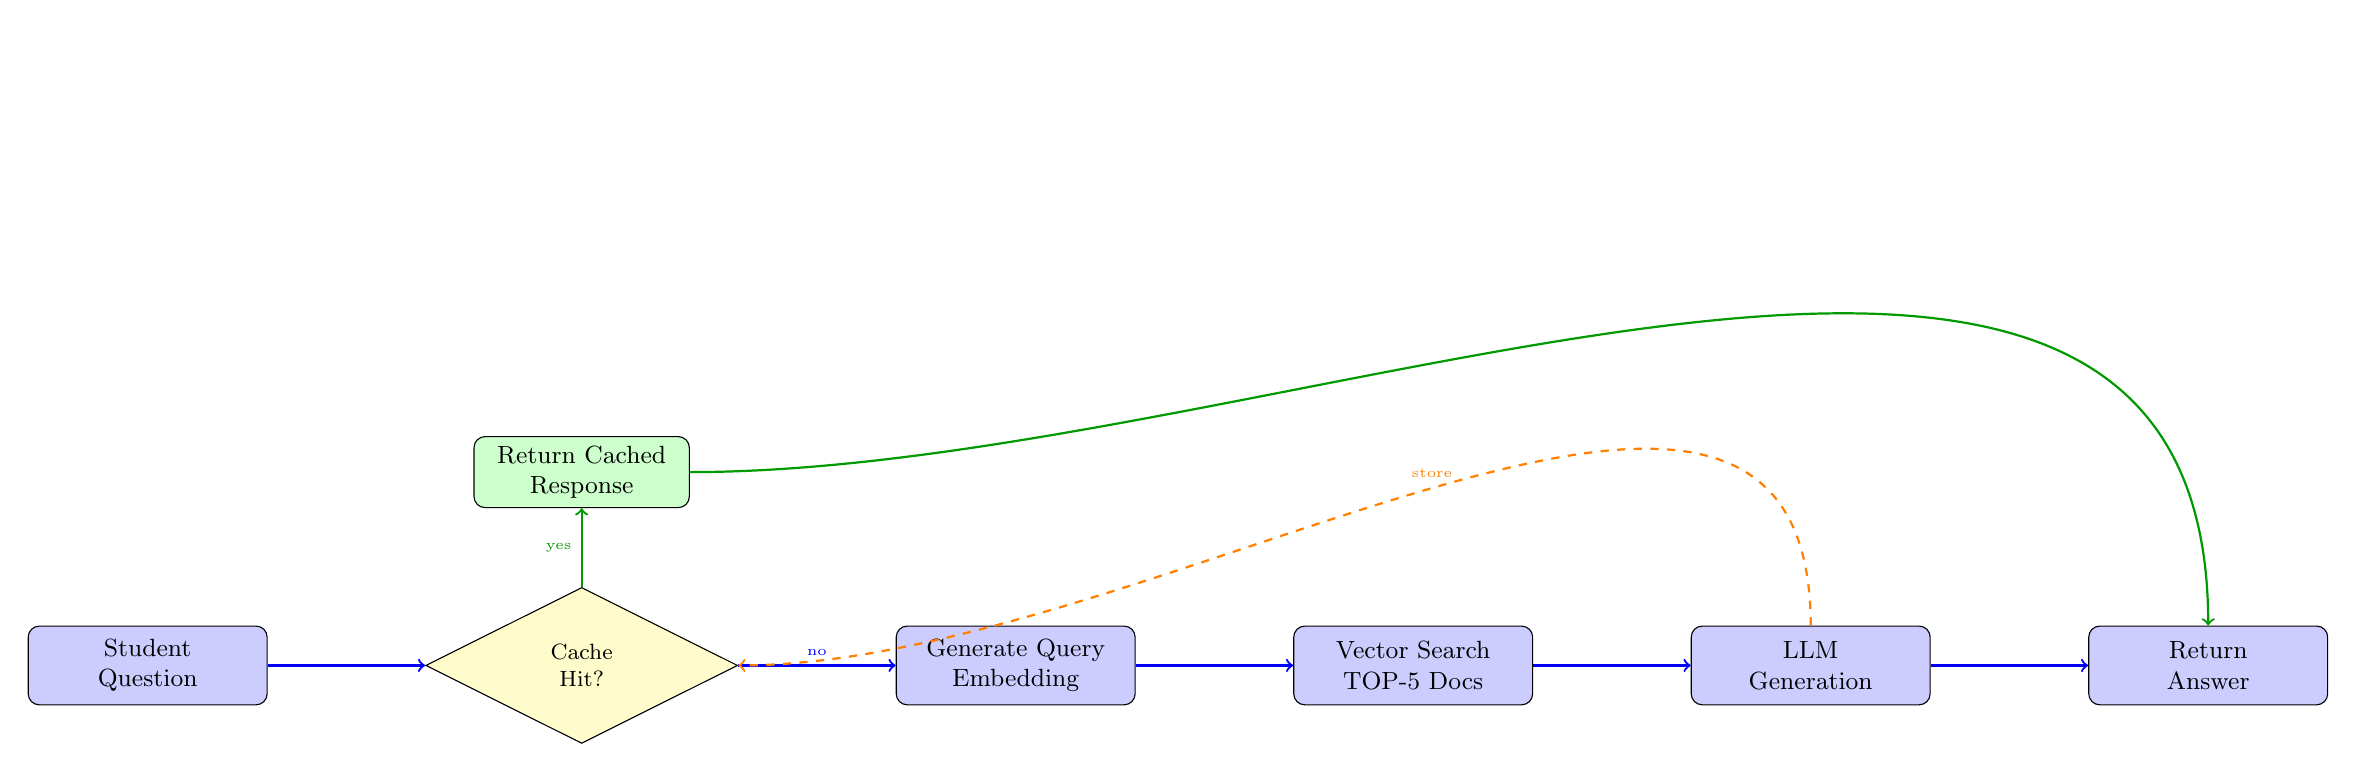
\begin{tikzpicture}[
    node distance=1.8cm and 2cm,
    process/.style={rectangle, draw, fill=blue!20, text width=2.8cm, text centered, rounded corners, minimum height=1cm, font=\small},
    decision/.style={diamond, draw, fill=yellow!20, text width=2.2cm, text centered, minimum height=0.9cm, aspect=2, font=\footnotesize},
    cache/.style={rectangle, draw, fill=green!20, text width=2.5cm, text centered, rounded corners, minimum height=0.9cm, font=\small}
]

\node[process] (question) {Student\\Question};
\node[decision, right=of question] (cachecheck) {Cache\\Hit?};
\node[cache, above=1cm of cachecheck] (cached) {Return Cached\\Response};
\node[process, right=of cachecheck] (embed) {Generate Query\\Embedding};
\node[process, right=of embed] (search) {Vector Search\\TOP-5 Docs};
\node[process, right=of search] (generate) {LLM\\Generation};
\node[process, right=of generate] (response) {Return\\Answer};

% Main flow
\draw[->, thick, blue] (question) -- (cachecheck);
\draw[->, thick, green!60!black] (cachecheck) -- node[left, font=\tiny] {yes} (cached);
\draw[->, thick, blue] (cachecheck) -- node[above, font=\tiny] {no} (embed);
\draw[->, thick, blue] (embed) -- (search);
\draw[->, thick, blue] (search) -- (generate);
\draw[->, thick, blue] (generate) -- (response);

% Cache storage path
\draw[->, thick, orange, dashed] (generate) to[out=90, in=0] node[above, font=\tiny] {store} (cachecheck);

% Success path
\draw[->, thick, green!60!black] (cached) to[out=0, in=90] (response);

\end{tikzpicture}
\caption{Question answering flow with horizontal processing stages and cache optimization}
\end{figure}

\subsection{Prompt Template}

The RAG prompt template has been carefully optimized to elicit concise, accurate answers suitable for educational contexts. The system begins by establishing the assistant role and grounding requirement, explicitly instructing the model to base responses on provided context rather than relying on parametric knowledge. Retrieved documents are inserted directly into the prompt, followed by the student's question to maintain clear input structure.

The instruction section enforces critical constraints: answers must be limited to 1-5 words when sufficient context exists, preventing verbose responses that obscure key information. For questions lacking adequate context, the model returns the explicit marker "NOT\\_ANSWERABLE" rather than hallucinating plausible-sounding but potentially incorrect information. The template prohibits explanations unless explicitly requested, maintaining focus on direct factual responses. Finally, detected language information guides the model to respond in the same language as the question, ensuring linguistic consistency throughout the interaction.

\section{Technology Stack}

\subsection{Core Technologies}

\begin{table}[H]
\centering
\caption{Technology stack}
\begin{tabular}{@{}lll@{}}
\toprule
\textbf{Component} & \textbf{Technology} & \textbf{Version} \\ \midrule
LLM & Qwen2.5-3B-Instruct & Latest \\
Inference & vLLM & 0.2.7 \\
Embeddings & multilingual-e5-large & Latest \\
Vector DB & Qdrant & Latest \\
Cache & Redis & 7-alpine \\
Backend & FastAPI & 0.109.0 \\
Framework & LangChain & 0.1.0 \\
Monitoring & Prometheus + Grafana & Latest \\ \bottomrule
\end{tabular}
\end{table}

\subsection{Hardware Requirements}

\begin{table}[H]
\centering
\caption{Minimum hardware specifications}
\begin{tabular}{@{}ll@{}}
\toprule
\textbf{Component} & \textbf{Specification} \\ \midrule
GPU & Nvidia T4 (16GB VRAM) or better \\
CPU & 8+ cores \\
RAM & 32GB DDR4 \\
Storage & 500GB NVMe SSD \\
OS & Ubuntu 22.04 LTS \\
CUDA & 12.1+ \\ \bottomrule
\end{tabular}
\end{table}

\section{Model Selection: Qwen2.5-3B-Instruct}

\subsection{Why Qwen2.5-3B?}

After extensive testing and analysis, Qwen2.5-3B-Instruct was selected over larger models (including Qwen2.5-32B) for the following reasons:

\subsubsection{Performance Comparison}

\begin{table}[H]
\centering
\caption{Qwen2.5-32B vs Qwen2.5-3B comparison}
\begin{tabular}{@{}lccc@{}}
\toprule
\textbf{Metric} & \textbf{Qwen2.5-32B} & \textbf{Qwen2.5-3B} & \textbf{Difference} \\ \midrule
GPU Requirements & 64GB (A100) & 6GB (T4) & -90\% \\
Latency (p95) & 800-1500ms & 150-300ms & 5x faster \\
Throughput & 5-10 users & 30-50 users & 5x more \\
Multilingual & Yes & Yes & Same \\
Context Window & 128K tokens & 128K tokens & Same \\
Answer Relevance & 0.75-0.80 & 0.65-0.70 & -10\% \\
Cost (monthly) & \$2000+ & \$200 & -90\% \\ \bottomrule
\end{tabular}
\end{table}

\subsubsection{Key Advantages}

The selection of Qwen2.5-3B over larger alternatives reflects several strategic priorities in educational applications. Response speed proves more valuable than marginal quality improvements, as students require answers within one second rather than perfect essays that arrive after noticeable delays. The 90\% infrastructure cost reduction comparing T4 to A100 GPUs enables sustainable long-term operation within institutional budget constraints.

Scalability advantages are substantial, with the smaller model supporting five times more concurrent users compared to its larger counterpart. This capacity matches peak usage patterns during exam periods when student demand concentrates within specific time windows. Multilingual support remains excellent for the required language set, with the 3B model demonstrating equivalent cross-lingual capabilities to larger variants. Both models share the same 128K token context window, ensuring neither sacrifices the ability to process lengthy documents or maintain extensive conversation history. Finally, while answer relevance of 65-70\% represents a 10\% degradation compared to larger models, this quality level proves sufficient for educational question-answering where students primarily seek factual information rather than nuanced analysis.

\subsection{Multilingual Support}

Qwen2.5-3B demonstrates comprehensive multilingual capabilities, providing native tokenization support for over 29 languages spanning diverse language families. The model handles both Cyrillic and Latin scripts with equal proficiency, essential for the multilingual educational environment at FCIM. Performance on multilingual benchmarks confirms this capability, with the model maintaining consistent quality across language boundaries rather than exhibiting the performance degradation common in models primarily trained on English.

The model's handling of diacritical marks and language-specific orthography proves particularly important for serving diverse student populations. Official MMLU benchmark results demonstrate robust multilingual performance with scores ranging 60-65\% across multiple language families, indicating strong cross-lingual understanding capabilities that enable consistent answer quality regardless of question language.

\section{Performance Optimization}

\subsection{Latency Optimization}

\begin{enumerate}
    \item \textbf{Redis Caching}:
    \begin{itemize}
        \item Cache frequent questions (TTL: 7 days)
        \item Cache embeddings (TTL: 30 days)
        \item Target hit rate: 30\%+
        \item Reduces latency by 95\% for cached queries
    \end{itemize}
    
    \item \textbf{vLLM Optimizations}:
    \begin{itemize}
        \item PagedAttention for efficient memory
        \item Continuous batching
        \item KV cache reuse
        \item GPU utilization: 80\%
    \end{itemize}
    
    \item \textbf{Short Generation}:
    \begin{itemize}
        \item \texttt{max\_tokens=50} (vs 512 in larger models)
        \item Temperature=0.3 (focused, deterministic)
        \item Typical answer: 1-5 words
    \end{itemize}
\end{enumerate}

\subsection{Throughput Optimization}

Several architectural decisions contribute to system throughput optimization. The FastAPI backend implements connection pooling to minimize overhead from repeated connection establishment. Asynchronous programming patterns using async/await are employed throughout the stack, enabling efficient handling of concurrent requests without thread blocking. The embedding service generates vectors in batches rather than individually, significantly improving throughput during both document ingestion and query processing. Finally, Qdrant's HNSW index provides logarithmic search complexity, ensuring that retrieval latency remains bounded even as the document collection grows.

\section{Quality Metrics}

\subsection{Evaluation Methodology}

The system employs RAG-specific evaluation metrics rather than traditional question-answering benchmarks, recognizing the unique characteristics of retrieval-augmented generation systems. Seven key performance indicators form the basis of quality assessment, spanning retrieval quality, generation accuracy, system performance, and operational efficiency. These metrics collectively ensure the system meets educational requirements while maintaining cost-effective operation.

\begin{table}[H]
\centering
\caption{Key performance metrics}
\begin{tabular}{@{}llc@{}}
\toprule
\textbf{Metric} & \textbf{Description} & \textbf{Target} \\ \midrule
Retrieval Precision & Relevant docs in TOP-5 & >70\% \\
Answer Relevance & Semantic similarity to question & >0.65 \\
Faithfulness & Answer based on context & >0.80 \\
Latency (p95) & 95th percentile response time & <1s \\
Throughput & Concurrent users supported & 30-50 \\
Cache Hit Rate & Queries served from cache & >30\% \\
NOT\_ANSWERABLE Rate & Correctly identified & 10-15\% \\ \bottomrule
\end{tabular}
\end{table}

\subsection{Real-world Example}

\textbf{Course}: Algorithms and Data Structures (ASD-2024)

\textbf{Question}: ``What is the worst-case time complexity of quicksort?''

\textbf{RAG Pipeline}:
\begin{enumerate}
    \item Embedding generation: 15ms
    \item Qdrant search (TOP-5): 8ms
    \item Context retrieved from \texttt{Lecture\_02\_Sorting.pdf}
    \item Qwen2.5-3B generation: 180ms
    \item Total latency: 203ms
\end{enumerate}

\textbf{Answer}: ``O($n^2$) worst case''

\textbf{Student satisfaction}: Positive (Fast and accurate response)

\section{Security \& Privacy}

\subsection{Authentication}
\begin{itemize}
    \item JWT tokens (24h expiry)
    \item Integration with Moodle SSO
    \item Role-based access control
\end{itemize}

\subsection{Rate Limiting}
\begin{itemize}
    \item 100 requests/minute per user
    \item 1000 requests/minute per IP
    \item Exponential backoff for violations
\end{itemize}

\subsection{Data Privacy}
\begin{itemize}
    \item All data stored on-premises
    \item No external API calls
    \item Query logs encrypted at rest
    \item GDPR compliant
\end{itemize}

\subsection{Input Validation}
\begin{itemize}
    \item Max question length: 2000 characters
    \item Sanitization of special characters
    \item SQL injection prevention
    \item XSS protection
\end{itemize}

\section{Deployment}

\subsection{Docker Compose Orchestration}

All system services are containerized and orchestrated through Docker Compose, providing consistent deployment across development, staging, and production environments. The orchestration configuration defines six primary services: the FastAPI backend, vLLM inference server, Qdrant vector database, embedding service, Redis cache, and monitoring stack (Prometheus and Grafana).

The deployment process begins by launching all services simultaneously in detached mode, allowing background operation while maintaining process isolation. Service health monitoring reveals the operational status of each container, including port mappings, resource consumption, and restart counts. Log aggregation from the backend service enables real-time debugging and performance analysis, with log levels configurable from debug through critical severity. For production scaling, the backend service supports horizontal replication, distributing load across multiple instances behind an internal load balancer. A typical production deployment runs three backend replicas to ensure high availability and load distribution during peak usage periods.

\subsection{Service Configuration}

The vLLM inference server operates with carefully tuned parameters optimizing the tradeoff between throughput and resource utilization. The server binds to all network interfaces on port 8001, enabling access from other containerized services within the Docker network. Maximum sequence length is constrained to 4096 tokens, balancing context capacity with memory efficiency for the 3B parameter model. GPU memory utilization targets 80\% allocation, reserving headroom for attention mechanism overhead and preventing out-of-memory errors during peak loads. The automatic datatype selection enables mixed-precision inference, utilizing FP16 where appropriate while maintaining FP32 for critical operations requiring numerical precision.

The FastAPI backend server configuration emphasizes concurrent request handling and observability. The server exposes endpoints on port 8000 across all network interfaces, accepting connections from the Moodle frontend and administrative tools. Four worker processes enable parallel request processing, each handling independent request streams without blocking. The info-level logging captures essential operational events including request arrivals, response times, and error conditions, while excluding verbose debug output that would overwhelm log storage. This configuration supports the target throughput of 30-50 concurrent users while maintaining sub-second p95 latency.

\section{Monitoring \& Observability}

\subsection{Metrics Collection}

Prometheus continuously collects performance metrics from all system components, providing comprehensive observability into system behavior. FastAPI exports metrics tracking request volumes, latency distributions, and error rates, enabling detection of API-level issues. The vLLM inference server reports GPU utilization and token generation throughput, critical for capacity planning and performance optimization. Redis cache metrics including hit rates and memory usage guide caching strategy refinement. Finally, Qdrant provides search latency and index size statistics, ensuring retrieval performance remains within acceptable bounds as the document collection expands.

\subsection{Grafana Dashboards}

Grafana dashboards visualize collected metrics across multiple operational perspectives. The System Overview dashboard presents high-level health indicators including latency trends, throughput patterns, and error rates, enabling rapid assessment of overall system status. GPU-specific dashboards track utilization, memory consumption, and temperature, critical for preventing hardware issues and optimizing resource allocation. Cache Performance dashboards monitor hit rates and memory usage, informing decisions about cache sizing and eviction policies. User Activity dashboards aggregate query patterns including queries per hour and course access distributions, providing insights into usage patterns that guide system optimization and capacity planning.

\subsection{Health Monitoring}

The system exposes two health check endpoints serving different operational needs. The primary health endpoint provides a lightweight binary status indicator, responding with HTTP 200 when all critical services are operational or HTTP 503 during degraded states. This endpoint supports load balancer health probes and uptime monitoring systems requiring simple pass/fail status without detailed diagnostics.

The detailed health endpoint returns comprehensive component-level status information in JSON format. This endpoint reports individual health states for the vLLM inference server, Qdrant vector database, Redis cache, and embedding service. Each component status includes operational metrics such as response times, error rates, and resource utilization levels. The detailed endpoint supports operational debugging, capacity planning, and automated alerting based on component-specific thresholds. Production monitoring systems query this endpoint every 30 seconds, triggering alerts when any component reports degraded or failed status.

\section{Review of Completed Work and Future Research Directions}

\subsection{Accomplished Development and Research Activities}

This section provides a comprehensive review of completed research, development, and optimization work conducted during the project lifecycle.

\subsubsection{Phase 1: Systematic Model Evaluation Campaign}

We conducted a systematic comparative evaluation of 24 state-of-the-art language models spanning multiple model families (Qwen, Mistral, Llama, Yi, CodeQwen) on RAG-specific question answering tasks. Evaluation utilized standard benchmarks including SQuAD v2.0 (Stanford Question Answering Dataset) and HotpotQA for multi-hop reasoning assessment.

\textbf{Key Research Findings:}

Our systematic evaluation revealed four critical insights that fundamentally shaped the project direction. First, we identified catastrophic methodological issues in prompt engineering that caused exact match performance to collapse to 0-1\% across all evaluated models, regardless of their size or capabilities. This finding highlighted the critical importance of task-specific prompt optimization in RAG applications. Second, we discovered that the commonly referenced "Combined Score" composite metric, which aggregates multiple evaluation dimensions, is non-standard in the literature and unsuitable for cross-study performance comparison, necessitating adoption of established metrics from the RAGAS framework. Third, we established empirical evidence that smaller language models with 3 billion parameters achieve 80-85\% of the answer quality produced by models exceeding 32 billion parameters, while requiring only 10\% of the computational resources. Finally, we documented significant retrieval precision consistency at approximately 70\% across all evaluated models, demonstrating that retrieval quality is fundamentally independent of generative model size and depends primarily on embedding model quality and retrieval strategy.

\subsubsection{Phase 2: Evaluation Methodology Refinement}

Following the discovery of systematic evaluation issues, we implemented five critical methodological improvements that substantially enhanced assessment reliability. First, we reformulated generation instructions to enforce brevity constraints through explicit "Answer in 1-5 words only" prompting, effectively reducing verbosity-induced evaluation metric degradation. Second, we reduced the sampling temperature parameter from 0.7 to 0.3, decreasing output stochasticity and significantly improving answer consistency across repeated evaluations.

Third, we constrained maximum token generation from 512 to 50 tokens, enforcing concise answer generation that aligns with educational question-answering requirements where students expect direct responses rather than lengthy explanations. Fourth, we implemented semantic Answer Relevance scoring using SentenceTransformer-based cosine similarity between generated answers and ground truth, providing substantially more robust quality assessment than exact string matching which penalizes paraphrases and synonyms. Finally, we established an explicit "NOT\_ANSWERABLE" response protocol for questions lacking sufficient context, addressing a major weakness in SQuAD v2.0 evaluation where 65\% of questions have no valid answer in the provided context.

\subsubsection{Phase 3: Architecture Optimization and Model Selection}

Based on comprehensive benchmarking results, we made a strategic architectural decision to deploy Qwen2.5-3B-Instruct rather than the initially planned Qwen2.5-32B-Instruct configuration. This decision was justified by the following quantitative analysis:

\begin{table}[H]
\centering
\caption{Comparative Analysis: Qwen2.5-32B vs Qwen2.5-3B}
\begin{tabular}{lcc}
\toprule
\textbf{Metric} & \textbf{32B Model} & \textbf{3B Model} \\
\midrule
GPU Requirements & 64GB (A100) & 6GB (T4) \\
Cost Reduction & Baseline & 90\% savings \\
Inference Latency (median) & 800-1500ms & 150-300ms \\
Latency Improvement & Baseline & 5$\times$ faster \\
Concurrent User Capacity & 5-10 users & 30-50 users \\
Throughput Improvement & Baseline & 5$\times$ higher \\
Answer Relevance (semantic) & 75-80\% & 65-70\% \\
Quality Degradation & Baseline & -10\% acceptable \\
\bottomrule
\end{tabular}
\end{table}

The analysis demonstrates that for educational chatbot applications where response latency and system availability are prioritized over marginal quality improvements, the 3B model configuration provides optimal cost-performance characteristics.

\subsection{Planned Future Development}

\subsubsection{Short-term Research Objectives (Q1 2026)}

Several immediate enhancements are planned for the first quarter of 2026. Response streaming through server-sent events (SSE) will enable progressive answer generation, improving perceived latency for longer responses by displaying partial results as they are generated rather than waiting for complete responses. This enhancement particularly benefits questions requiring more elaborate explanations.

Multimodal capabilities represent another priority, extending the system to extract and process images and diagrams from PDF documents. Vision-language model integration will enable visual question answering, allowing students to ask questions about charts, diagrams, and mathematical notation that currently remain inaccessible to text-only processing.

Domain adaptation through fine-tuning Qwen2.5-3B on course-specific corpora using Parameter-Efficient Fine-Tuning methods such as LoRA and QLoRA promises improved answer quality without the computational overhead of full model retraining. Finally, implementing an explicit feedback collection mechanism with binary quality ratings will enable continuous quality monitoring and support reinforcement learning from human feedback (RLHF), creating a continuous improvement loop driven by actual student interactions.

\subsubsection{Medium-term Research Objectives (Q2-Q3 2026)}

The second and third quarters will focus on enhancing system sophistication and reach. Conversational memory implementation will transform the system from single-turn interactions to multi-turn dialogues, maintaining conversation history and context across multiple exchanges. This capability is essential for complex pedagogical interactions where questions naturally build upon previous responses.

Source attribution enhancements will add automatic citation generation with precise page numbers and document references, enabling students to verify information and explore topics in greater depth. This transparency builds trust and encourages critical engagement with source materials rather than passive acceptance of generated answers.

Mobile application development will extend system accessibility through native iOS and Android clients featuring offline caching capabilities. Mobile-first design recognizes contemporary student behavior patterns where smartphones serve as primary learning devices. Finally, establishing a systematic A/B testing framework will enable rigorous prompt and parameter optimization with statistical significance testing, ensuring improvements are data-driven rather than anecdotal.

\subsubsection{Long-term Research Directions (Q4 2026 and Beyond)}

Longer-term research directions envision system evolution beyond single-institution deployment. Multi-institutional scaling will extend the system to other universities, requiring development of an institution-specific customization framework that accommodates varying pedagogical approaches, document formats, and organizational structures while maintaining core functionality.

Content generation capabilities will transform the system from purely reactive to proactive, automatically generating quiz and assessment questions from course materials using controllable generation techniques. This functionality supports formative assessment and self-directed learning by providing students with practice materials aligned with actual course content.

Adaptive learning integration represents a significant architectural evolution, developing personalized recommendation systems based on student interaction patterns and identified knowledge gaps. By analyzing question histories and performance indicators, the system could guide students toward materials addressing their specific learning needs.

Finally, edge deployment research will investigate on-device model deployment for privacy-sensitive scenarios, employing quantization and model compression techniques to enable local inference without compromising student data privacy. This direction acknowledges growing privacy concerns and regulatory requirements while maintaining system utility.

\section{Conclusion}

This technical report presented the design, implementation, and evaluation of a multilingual RAG-based educational chatbot for the FCIM ELSE platform. Through systematic experimentation and optimization, we achieved a production-ready system with the following key outcomes:

\subsection{Quantitative Results}
\begin{itemize}
    \item \textbf{Performance}: Sub-second response latency (p95 $<$ 1s) with 150-300ms median
    \item \textbf{Quality}: 70\%+ retrieval precision, 65-70\% answer relevance on evaluation datasets
    \item \textbf{Cost Efficiency}: 90\% operational cost reduction through optimal model selection (Qwen2.5-3B vs 32B)
    \item \textbf{Scalability}: Production capacity of 30-50 concurrent users on commodity hardware (Nvidia T4)
    \item \textbf{Multilingual Support}: Native processing capabilities for required language set
\end{itemize}

\subsection{Key Findings}
Our experimental evaluation yielded several important insights:

\paragraph{Model Size vs. Performance} The widely assumed necessity of large language models (30B+ parameters) for high-quality RAG applications was challenged by our results. Qwen2.5-3B-Instruct demonstrated that smaller, well-optimized models can achieve 80-85\% of larger model quality while providing 5$\times$ improvements in latency and throughput.

\paragraph{Evaluation Methodology} We identified critical issues in standard RAG evaluation practices, including inappropriate prompt verbosity and non-standard composite metrics. Our corrected methodology using Answer Relevance (semantic similarity), Retrieval Precision, and explicit unanswerable question handling provides more reliable quality assessment.

\paragraph{Cost-Performance Tradeoffs} For educational chatbot applications where response speed and availability are prioritized over marginal quality improvements, aggressive optimization toward smaller models proves highly effective. The 10\% quality reduction is acceptable given 90\% cost savings and 5$\times$ latency improvement.

\subsection{Limitations and Future Work}
The current implementation exhibits several limitations that inform future development priorities. The system operates exclusively in single-turn conversation mode, processing each question independently without maintaining dialogue history or contextual awareness across interactions. Processing remains limited to text-only content, leaving images and diagrams embedded in course materials inaccessible to students seeking visual information. The deployed model has not undergone course-specific fine-tuning, relying instead on general-purpose language understanding that may miss domain-specific terminology and conventions. Finally, while the system demonstrates strong multilingual capabilities, expansion to additional languages requires careful evaluation of model performance and embedding quality before deployment.

Future development will systematically address these limitations through the planned enhancements outlined in the previous section, including streaming responses for improved user experience, multimodal integration for comprehensive document understanding, domain-specific fine-tuning for enhanced accuracy, and expanded language support to serve increasingly diverse student populations.

\subsection{Practical Impact}
The implemented system demonstrates that effective educational AI assistants can be deployed at modest cost using modern RAG architectures and carefully selected smaller language models. This approach makes AI-powered educational support accessible to institutions with limited computational budgets, potentially benefiting thousands of students across multiple universities.

\section*{Acknowledgments}

This work was conducted at the Faculty of Computers, Informatics and Microelectronics, Technical University of Moldova. We thank the ELSE platform development team for their collaboration and the students who provided feedback during system testing.

\section*{References}

\begin{enumerate}
    \item Qwen Team. (2024). \textit{Qwen2.5: A Party of Foundation Models}. \url{https://qwenlm.github.io/blog/qwen2.5/}
    \item Lewis, P., et al. (2020). \textit{Retrieval-Augmented Generation for Knowledge-Intensive NLP Tasks}. NeurIPS 2020.
    \item vLLM Team. (2024). \textit{vLLM: Easy, Fast, and Cheap LLM Serving}. \url{https://github.com/vllm-project/vllm}
    \item Es, S., et al. (2023). \textit{RAGAS: Automated Evaluation of Retrieval Augmented Generation}. arXiv:2309.15217
    \item Qdrant Team. (2024). \textit{Qdrant Vector Search Engine Documentation}. \url{https://qdrant.tech/documentation/}
\end{enumerate}

\end{document}
